\chapter{Fabrication \& Sensing of Input Devices}


\begin{quote}
If you think in terms of a year, plant a seed; if in terms of ten years, plant trees; if in terms of 100 years, teach the people.

--- Confucius
\end{quote}
\valkyrie{c'mon, need a better quote.}

\valkyrie{Consider using Klemmer's framework as an inspiration here. Consider organizing just around sensing principles and not worrying about enumerating machine properties in the same way. Don't necessarily use 5 human senses, but consider looking into a list of "common sensor types" that can be leveraged for organizational purposes. Still want to have a section about what machines can/can't do today, but probably easier to just keep these as shorter definitions and not worry about organizing them hierarchically or anything. should I combine RW and this chapter together?????}

%\begin{quote}
%The design of human-machine dialogues is, at least in part, the design of artificial languages for [human-machine] communication. [W]e can analyze the manipulations of an input device as sentences. Input devices are those devices that allow some portion of these potential sentences actually to be realized and communicated from human to machine.

%--- Stuart Card, et al.
%\end{quote}

This chapter outlines the multitude of digital fabrication techniques currently available, as well as potential characteristics of the artifacts that each process can create. We then align these properties to sensing techniques, describing a space of possible geometry/sensing links for input device design and fabrication.

\valkyrie{organize around 5 human senses?? this leaves out things like magnetic sensing (but we can have an ``other'' bucket?)}

\section{Definitions}

First, we briefly define uncommon words and machines that will be discussed in this chapter.

\emph{additive fabrication} : in additive fabrication, material is deposited and a shape is built up, leaving no waste

\emph{subtractive fabrication} : a subtractive fabrication process removes material to create a form. Excess material may be reused in another project or discarded.

\emph{3D printer} : a 3D printer is one of a class of machines that additively create a three-dimenstional model from one or more materials.

\emph{FFF} : FFF (fused-filament fabrication) 3D printers lay down material by melting and depositing a filament in a precise pattern.

\emph{model material} : model material is the substrate that the final object is made from

\emph{support material} : many modern 3D printers are capable of laying two types of materials, model material and a secondary, sacrificial material that can support overhangs in the model while printing, then be removed.

\emph{SLA} : SLA (stereolithography) printers use a bath of UV-curable polymer and a controllable UV laser. The laser "draws" each layer on the polymer, converting it from liquid to solid where it cures. Excess material is simply poured out for reuse.

\emph{SLS} : SLS (selective laser sintering) 3D printers contain a bed of material (e.g., metal powder) which is melted by a laser and rapidly cools into a solid, fused form. Excess material can be brushed off and reused.

\emph{PolyJet} : PolyJet printers have print heads similar to those of inkjet printers which sweep across the build area depositing material. Following the printer head is a UV light, which cures deposited material droplets.

\emph{vinyl cutter} : a vinyl cutter subtractively processes 2D materials with a 2-axis knife blade, cutting patterns into them. Vinyl cutters are typically used for thin, flexible materials.

\emph{laser cutter} : a laser cutter has a 2-axis laser for processing flat materials. Laser cutters can cut or etch into materials, and are often used for rigid, medium-thickness materials. Some have rotary attachments for etching on circular surfaces like the outside of a glass.

\emph{CNC router} : a CNC router uses a 2-axis rotary mill to cut through thick, rigid materials, like wood or certain metals. Some CNC routers are portable and can attach to many materials, while some are stationary with beds into which material is loaded.

\emph{CNC mill} : a CNC mill is a multi-axis machine which subtractively creates a 3D shape from a block of material, usually metal or wood.

\section{Digital Fabrication}

Digital fabrication machines are those which can take as input a digital design file, in 2D or 3D, and output a physical realization of that design; these machines stand in contrast to traditional crafting techniques (which are guided by the craftsperson, and take no design file) as well as manufacturing techniques (which require ``tooling'' for each design created). The true power of digital fabrication lies in its ability to create unique objects with each machine run \emph{without} the extensive setup and tooling necessary to change the product created by, for example, an injection moulding machine. This comes with the blessing and curse that each instance of an object costs as much to manufacture as the one before it, but allows for variations between instances without additional cost. For example, doctors can now create custom 3D printed replacement joints that fit patients' bodies \cite{findref}.

The joint interests of industry, academia, and hobbyist makers have led to a flourishing ecosystem of digital fabrication and rapid prototyping (RP) machines. These machines describe a continuum from simple vinyl cutters that can subtractively create 2-dimensional stickers to sophisticated multi-material 3D printers that can create multicolor and conductive designs that are fully 3D inside and out. These machines allow their manufactured products to achieve various structural and material properties. We examine these achievable properties, describing possible geometries, materials/properties, and assembly characteristics (see Table \ref{table:properties}).

\valkyrie{You can just, I guess, give a short definition of what each of these properties are, and then make a good table that shows which machines can create which geometries.}

\begin{table}
\begin{center}
\begin{tabular}{rll}
\textbf{FEATURE}& \textbf{MANIFESTATION} & \textbf{POSSIBLE MACHINES} \\
\textbf{geometry} & $2D$ & vinyl cutter, paper cutter, inkjet printer \\
& $2.5D$ & laser cutter, CNC router \\
& $3D$ external & CNC mill, 3D printer \\
& $3D$ internal + external & 3D printer \\
\textbf{materials} & plastic & laser cutter, 3D printer \\
& metal & vinyl cutter, 3D printer, CNC mill \\
& wood & laser cutter, CNC router \\
& vinyl & vinyl cutter, laser cutter \\
& paper & paper cutter, laser cutter \\
\textbf{properties} & inert & \\
& adhesive & \\
& flexible & \\
& stiff & \\
& conductive & \\
& blended & \\
& multi-colored & \\
& transparent & \\
\end{tabular}
\end{center}
\caption{Digital fabrication enables fabrication of a wide variety of geometries with different material and structural properties. \valkyrie{I still hate this table. Could work as something more like the other table (i.e., made in illustrator, with pix).}}
\label{table:properties}
\end{table}

\subsection{Geometry Fabrication}

Digital fabrication machines can support any complexity of geometry, from 2D images on paper (as an inkjet printer produces) to 3D projections of 4D objects (like Shapeways's Klein bottles printed in steel) (see Figure \ref{fig:range}. We describe the possibilities for the various geometries, as well as machines that could produce them. Note that we list machines at the edge of their range: for example, a CNC mill (listed under 3D external) can also make 2.5D or 2D objects.

\subsubsection{2D geometry}

2D geometry lies flat on a surface, but can manifest as an image printed on paper, a sticker cut from vinyl, or a barcode etched on granite. Machines that support 2D geometry fabrication include vinyl and paper cutters, as well as inkjet printers.

\subsubsection{2.5D geometry}

A slight jump from 2D is 2.5D: a 2D shape with additional \emph{depth} information. The canonical machines to create 2.5 objects are laser cutters (which can take multiple passes or vary laser strength to create different depths).

\subsubsection{3D external geometry}

\subsubsection{3D internal geometry}

\subsection{Materials and Properties}

\subsubsection{Plastic (hard)}

\subsubsection{Plastic (flexible)}

\subsubsection{Plastic (transparent)}

\subsubsection{Metal (conductive)}

\subsubsection{Metal (inert)}

\subsubsection{Wood}

\subsubsection{Vinyl (flexible)}

\subsubsection{Paper}

\subsection{Assembly Characteristics}

\section{Single-Sensor Sensing Techniques}

The essence of Human Computer Interaction is a computer understanding a person's interactions. Thus, while many of the input techniques here could be used in, for example, machine-to-machine communication, we describe how a person's actions might create a usable control signal.

A ``single sensor'' can take many forms, ranging from a humble switch which opens and closes to a high-speed video camera which captures 2D visual information at 1000Hz to an accelerometer measuring G-forces in 3 directions.
\valkyrie{Card, et al., provide an analysis of the space of input devices based on what is sensed: position, $\Delta$position, angle, $\Delta$angle, force, $\Delta$force, torque, and $\Delta$torque \cite{card-input}. We use this to frame our discussion, but include additional senseable aspects: identity (of a user), bend/$\Delta$bend, and ???. We could also include, for example, \emph{intent}, which is the input of NLP voice systems like Siri, however these types of non-physical input are challenging to conceive of as a part of a physical input device and we therefore ignore them for now.}
We organize our discussion around five categories of common sensors: contact, non-contact, electrical, environmental, and biological. In these five categories, we discuss thirty common varieties of sensors, like capacitance sensors, hall effect sensors, voltage sensors, temperature sensors, and pulse sensors.

\valkyrie{In this section, again just give short definitions of what each sensor type does?}

\subsection{Contact sensors}

\subsection{Non-contact sensors}

\subsection{Electrical sensors}

\subsection{Environmental sensors}

\subsection{Biological sensors}

\section{Promising Overlaps}

The spaces of both machines and sensors are vast, so we describe some ways to think about combining them to actually fabricate sensing objects. \valkyrie{need to talk about every X in table? definitely need to talk generically about how you are defining something as "promising" here. :)}

\begin{figure}
\begin{adjustbox}{addcode={\begin{minipage}{\width}}{\caption{%
      Lining up the possibilities of fabricatable properties with sensor types, we can see several areas that are promising for further exploration. We also identify pairings that have been explored previously, as well as pairings explored in this thesis. \valkyrie{for previously explored, probably want to in some way tie to the works (i.e., with refs in figure).}
      }\end{minipage}},rotate=90,center}
      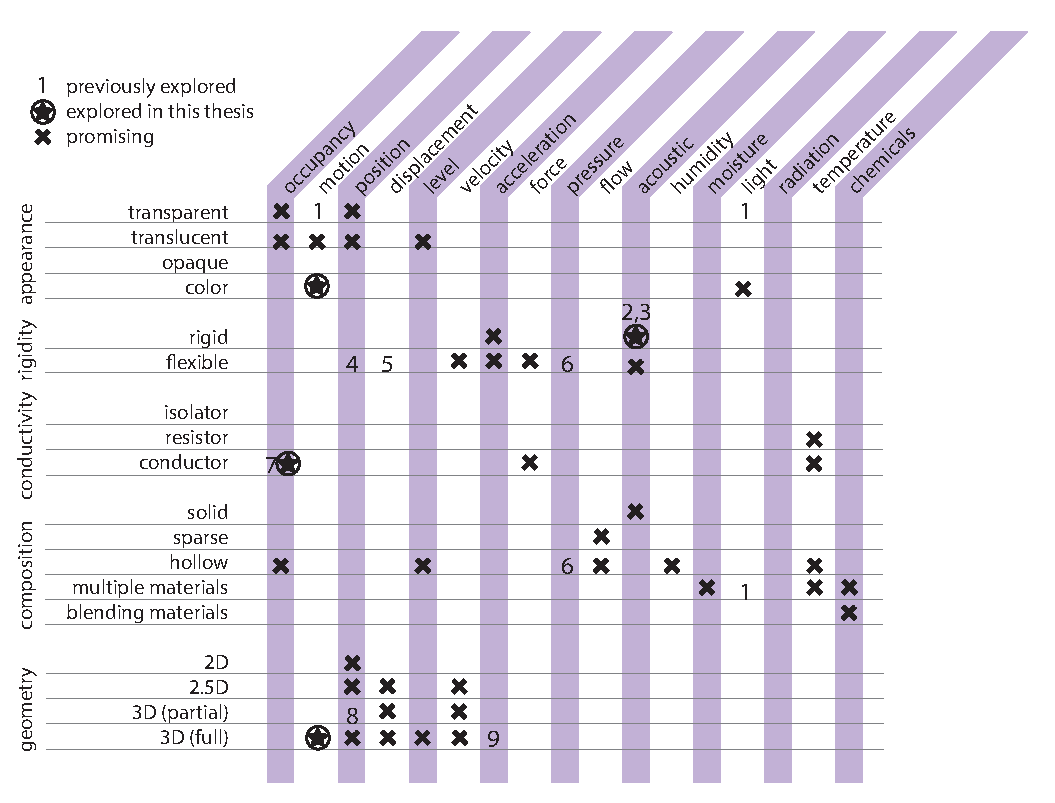
\includegraphics[scale=.8]{figures/sensing-fab.pdf}%
  \end{adjustbox}
\label{fig:sensing-fab}
\end{figure}